%!TEX root = ../script.tex

\section{Ethereum and Smart Contracts}

\noindent
Ethereum is a Proof of Work blockchain, very similar to BitCoin.
Ethereum has its own cryptocurrecy, \emph{ether}, and uses hashes of public keys as addresses and identities, as bitcoin does.
However Ethereum implements several of the optimizations mentioned earlier.

\begin{itemize}
	\item Ethereum has an average block delay of only 12 seconds.
	\item Ethereum uses a different P2P network, namely \href{https://pdos.csail.mit.edu/~petar/papers/maymounkov-kademlia-lncs.pdf}{Kademlia}.
	\item Ethereum uses a different PoW function,  \href{https://eth.wiki/concepts/ethash/design-rationale}{Ethash}, which aims for ASIC resistance, as discussed in Section~\ref{sec:asic-resistance}.
	\item Ethereum uses Uncles and the GHOST rule, as discussed in Chapter~\ref{ch:scaling}.
\end{itemize}

\subsection{SmartContract}
Ethereum is mainly known for enabling Smart Contracts. 
These allow to encode more complex logic than the scripts in Bitcoin, i.e. redeem conditions.

\begin{definition} A \textbf{Smart Contract} is similar to an object in OOP. 
It has fields (state) and methods (functions) and is stored on the blockchain.
Further, the contract is characterized by the following properties:
\begin{enumerate}
	\item The code (function implementation) is public and cannot be changed.
	\item Any user can invoke the functions and thus update the state.
	\item The contract object can own money (ether)
	\item Users can send money to the contract together with invoking functions.
	\item The contract can send money to other contracts or users, inside functions.
\end{enumerate}
\end{definition}

\begin{note}
Points~1 and~2 above ensure that strangers can use the same contract. If they verify the contract code, they don't need to trust the user that published the contract.

Points~3-~5 allow to couple sending of money with function invocation. This simplifies the integration of money flows into an application.
\end{note}

\subsection{Accounts}
\noindent
Ethereum does not use the UTXO model. Instead, Ethereum uses accounts.
Ethereum distinguishes between external and internal accounts.
For every account, the Ethereum nodes store the fields, \textbf{address}, \textbf{nonce}, \textbf{balance}, \textbf{storage root}, and \textbf{code hash}.

\begin{definition}
In Ethereum \textbf{external accounts} are accounts belonging to users or rather identified by a public key. For every external account, the following data is stored:
\begin{description}
	\item[address] The accounts identified, a hash of the public key.
	\item[balance] The amount of ether owned by this account.
	\item[nonce] The sequence number of the last transaction sent from this account.
\end{description}
Also external accounts have the fields \textbf{storage root} and \textbf{code hash}, but they are empty.
\end{definition}

\begin{definition}
A \textbf{internal account} or \textbf{contract account} is the address of a 
smart contract. It has the following fields:
\begin{description}
	\item[address] The accounts identified, derived from a hash of the contact creator address and the nonce of the transaction that created the contract.
	\item[balance] The amount of ether owned by this account.
	\item[nonce] The number of other contracts (accounts) created from this account.
	\item[storage root] The root hash of the storage, or state of the contract.
	\item[code hash] The hash of the contracts code.
\end{description}
\end{definition}

\begin{note}
Internal accounts have a storage root and code hash. However, while transactions can update the storage root, the code hash cannot be updated.	

There are proposals to include the code hash in the derivation of the address.
However, the code hash alone is not sufficient for derivation of the address, since two contracts may have the same code.
\end{note}

\subsection{Transactions}
Transactions in Ethereum are always invoked from an external account. 
Transactions can transfer money, invoke functions on smart contracts or both.

Transactions have the following fields:
\begin{description}
	\item[nonce] next sequence number for sender account
	\item[gas price] how much ether the sender is willing to pay per gas unit
	\item[max gas] the maximum gas consumption of the transaction
	\item[recipient] destination Ethereum address
	\item[value] amount of ether sent along with the transaction
	\item[data] payload send with transaction, e.g. function identifier and arguments
	\item[signature] the signature from the sender, including his public key
\end{description}

If the recipient is an externally owned account, the transaction simply transfers the \emph{value}.
If the recipient is a contract account, the \emph{data} is decoded to detect which function should be run, and with what parameters. If no function is matched, the default function is run.

As part of the function execution, a contract can call functions a different contract. This is called an \emph{internal transaction}. Internal transactions are always part of an external transaction.

\paragraph{Transaction validation}
When validating a transaction the following checks are done:
\begin{itemize}
	\item The \emph{nonce} is the next sequence number for the sender.
	\item The sender has sufficient funds to pay \emph{value} and \emph{fees}.
	\item The signature is correct.
\end{itemize}

\begin{note}
When validating a transaction, it is not checked that the transaction executes correctly. A function invocation that causes an error may still be part of a valid transaction, be executed and will cost fees.
\end{note}

In a smart contract, you can access the address of the sender as \texttt{msg.sender}. This allows the contract to authenticate the sender, relying on the signature check on the transaction.

\begin{note}
On internal transactions \texttt{msg.sender} will not indicate the address of the contract invoking the internal transaction.

\texttt{msg.origin} is available to show the sender of a transaction, to which an internal transaction belongs. However using this field may have security issues.
\end{note}

\subsection{Gas}
Fees in ethereum are calculated in \emph{Gas}.
The sending of a transaction, function invocation and every assembly operation has a specific (fixed) gas cost. 
When issuing a transaction, the sender specifies \emph{Gas price}, saying how much ether he is willing to pay per Gas unit.

Thus executing the same transaction costs the same amount of gas, but the actual fee may differ depending on the gas price.

Similar to Bitcoin, miners will include the transactions with the largest gas price, since also block size is given in gas.

\begin{note}
Requiring gas prevents users from staging a DOS attack by writing an infinite loop.
\end{note}

\paragraph{gas limit}
A transaction specifies a \emph{gas limit}, saying how much gas the transaction may use at most. If the gas limit is reached, the transaction is reverted.
However, the transaction will still be included in a block and executed, and thus will cost the sender fees.

\begin{note}
The \emph{gas limit} can be used to avoid unexpectedly high fees. 
The reason this is necessary is that other transactions may change the state of a contract, and state changes may affect the execution of a function/transaction.
\end{note}

\begin{example}
Assume a function iterates over a list. If other transactions insert elements into that list, executing the iterating function will be more expensive.
\end{example}

\paragraph{gas tuning and storage}
Since the invocation of transaction costs gas, it is common to optimize the gas usage of functions, since this will save users actual money.

Operations that need to allocate storage are extra expensive. 
That is because the values have to be stored by all Ethereum nodes, possibly forever.
Similar, if some elements are removed from storage, this actually costs a negative amount of gas.

\section{Smart Contract Security}
	See slides and \url{https://github.com/ethereumbook/ethereumbook/blob/develop/09smart-contracts-security.asciidoc}.
	
\section{Oracles}
Smart contracts do not have access to data hosted outside of the blockchain. 
This is significantly limiting their usefulness, since many application have the need to access real data.
For example
\begin{itemize}
	\item a sports-betting application needs access to match results.
	\item a financial application needs access to exchange rates.
	\item an insurance application needs to know wether an event occurred.
	\item an online-store application needs access to wether a good was shipped.
\end{itemize}

For some kind of information, e.g. exchange rates, weather data, ... trusted sources and web-apis exist. 
However it is not possible for a smart contract to make a https request.

This problem can be solved by using an oracle:
\begin{definition} An \textbf{oracle} is a special smart contract that published real world data onto the blockchain.
\end{definition}

\begin{example}\label{ex:oracle}
Assume we want to build an application, that allows event hosts (e.g. festivals) to ensure against bad weather. 
Our application would like to access both historical weather data and predictions from a public api like yr.no.

Figure~\ref{fig:oracle} shows the different components of the application.
It has the following components:
\begin{itemize}
	\item The \emph{insurance contract} includes application logic of our insurance.
	\item The \emph{oracle contract} can be called from the insurance contract, when access to the web-api is needed.
	The oracle contract will then emit an event.
	\item A web application, \emph{oracle web-app} listens for events from the oracle contract. Upon events this application invokes requests to the public api. It then invokes a function on the oracle contract with the requested data.
	The oracle contract calls a callback on the insurance contract.

\end{itemize}
\begin{figure}
	\centering
	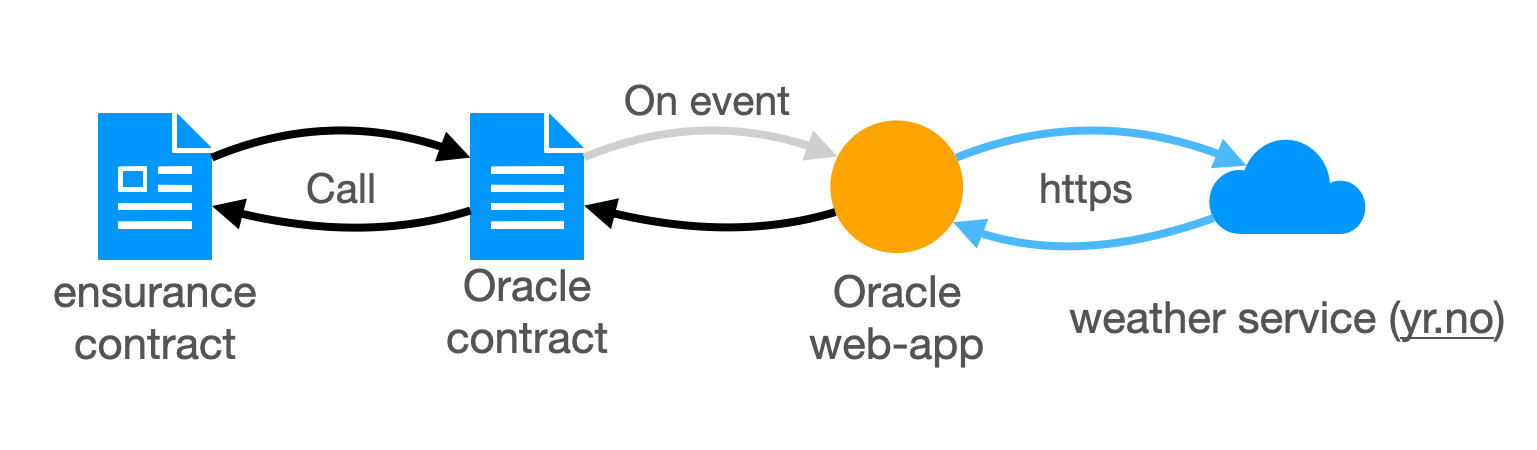
\includegraphics[width=0.8\textwidth]{fig/oracle-example}
	\caption{\label{fig:oracle}Oracle example.}
\end{figure}
\end{example}
\begin{note}
	An oracle is in itself a trusted source.
	In the architecture described in Example~\ref{ex:oracle}, the insurer and its client both need to trust the weather service, but also the oracle web app. 
	That is because the oracle web-app may falsify the information received from the weather service.
	
	The oracle contract is separated from the insurance contract, so that it can be replaced, if the oracle seems not trustful.
\end{note}

\paragraph{Improving trust}
There exist measures that can be used to increase trust in an oracle.

\begin{enumerate}
	\item Vote among multiple oracles.
	\item Use trusted hardware to run the oracle web-app, i.e. Intel SGX.
	\item Use zero-knowledge proofs (checked by oracle contract) to show that information was correctly received using https.
\end{enumerate}

\noindent
Point 1. has the advantage that it can also be applied, if no trusted web-api is available.
Points 2 and 3 are interesting, since they also allow to proof facts about private data, without revealing that data. In that case, the oracle web-app can be run by the owner of private data.


\section{Off chain transactions}
The idea behind off-chain transactions is to allow two parties to interact outside of the blockchain, i.e. without paying fees or waiting for long confirmation times. Only if the parties disagree on transactions, they use the blockchain to resolve the dispute.

This technique can mitigate the following problems:
\begin{description}
	\item[Fees] blockchain transactions incur high fees. They can therefore not be used for small, every day, transactions.
	\item[Scalability] the blockchain has a limited throughput and can therefore not handle all our every day transactions.
	\item[Confirmation time] blockchain transactions have long confirmation times, e.g. 1hour in bitcoin. They are thus not useful for everyday transactions.
\end{description}

\subsection{Uni-directional payment channel}
A unidirectional payment channel allows a payer $A$ to repeatedly transfer money to a payee $B$ off chain.

\begin{itemize}
	\item To open the channel, a smart contract is deployed. $A$ funds the contract with an initial balance $b$.
	\item $A$ can then send money to $B$ by simply sending $B$ a signed statement, including a balance $b_B\leq b$.
	\item $A$ can repeatedly send money to $B$ by sending another signed statement with an increased balance $b_B'> b_B$. However $b_B'\leq b$ must hold.
	\item $B$ can checkout his money, submitting the last balance $b_B'$, that he received from $A$ to the contract.
	\item Receiving the correctly signed balance $b_B''$ from $B$ the contract will payout $b_B''$ to $B$ and $b-b_B''$ to $A$.
\end{itemize}

The contract also has an expiration date. If $B$ does not submit a signed balance, before expiration, then $A$ can submit a transaction, terminating the contract and refunding $b$ to $A$.

\begin{note}
The benefit of an uni-directional payment channel is that it incurs fees only when opening and closing. Also, once the channel is opened, transfers can be confirmed by $B$ instantly, without waiting for the blockchain.

The drawback of uni-directional payment channels are:
\begin{itemize}
	\item The channel is limited by its initial balance. 
	\item The funds from $A$ are locked inside the channel. 
\end{itemize}	
\end{note}


\subsection{Bi-directional payment channel}
A bi-directional payment channel allows multiple off chain payments between $A$ and $B$, sending funds back and forth:

\begin{itemize}
	\item To open the channel, a smart contract is deployed. $A$ funds the contract with balance $b_A$ and $B$ funds the contract with balance $b_B$.
	\item To send $c$ funds to $B$, a creates a signed message with balances $b_A^1=b_A-c$, $b_B^1=b_B+c$ and an increasing sequence number $nonce=1$.
	\[
		\langle (b_A^1,b_B^1),1\rangle_{\sigma_A}
	\]
	\item $A$ and $B$ can repeatedly send money, by changing balances and increasing the nonce.
	\item To close the channel, $B$ can submit a message signed by both $A$ and $B$
	\[
		\langle (b_A^i,b_B^i),i\rangle_{\sigma_A,\sigma_B}
	\]
	When this happens, a predefined timeout is set.
	\item Before the timeout expires, $A$ can submit a balance with a higher nonce.
	\item After the timeout expires, $A$ and $B$ can withdraw their balance $b_A^i$.
\end{itemize}

\begin{note}
The bi-directional payment channel allows to send money back and forth. If the amount transferred from $A$ to $B$ is similar to the amounts transferred from $B$ to $A$, then many transactions can be sent back and forth.

One drawback of bi-directional channels is the need to define a timeout. 
A small timeout may be difficult to meet. Especially since blockchain transactions may see a lot of contention.
If timeouts are long, funds are locked.
Additionally both parties need infrastructure, to survey the blockchain and react within the timeout if necessary.
\end{note}

\subsection{Payment networks}
While payment channels can allow cheap transfer of funds, channels lock a users funds and the creation of channels is still subject to fees and the long confirmation time of the blockchain.

Therefore, creating channels with all users, that we send money to is not feasible. 

Payment networks allow to transfer funds across multiple channels.
Thus $A$ can send funds to $B$ without creating a channel, if the graph created by all channels includes a path from $A$ to $B$.

\begin{example}
Assume user $A$ maintains a channel to $X$, and user $B$ maintains a channel to $Y$. $X$ and $Y$ could for example be larger facilitators, e.g. banks.

Further we assume that a channel exists between $X$ and $Y$.
%
A payment can now be forwarded from $A$, via $X$ and $Y$ to $B$.

To transfer fund from $A$ to $B$ one can ask $Y$ and $X$ to forward such a payment. The smart contracts can be designed, such that, if $X$ promised to forward a payment, and received a payment from $A$, then forwarding to $Y$ can be enforced.
\end{example}
